\documentclass{beamer}
\mode<presentation>
{
	%\usetheme{CambridgeUS}
	\usetheme{Madrid}
	\usecolortheme{default}
	\usefonttheme{serif}
}
\usepackage[utf8]{inputenc}
\usepackage[russian]{babel}
\usepackage{cmap}
\usepackage{listings}
\usepackage{lmodern}
\usepackage{color}
\usepackage{minted}

\definecolor{links}{HTML}{2A1B81}
\hypersetup{colorlinks,linkcolor=,urlcolor=links}

\begin{document}
\title
[GlusterFS]
{GlusterFS}
\author
[Podkopaev Anton, Alexeyev Anton]
{
Podkopaev Anton, \texttt podkoav239@gmail.com\\
\and
Alexeyev Anton, \texttt anton.m.alexeyev@gmail.com
}
\institute[Computer Science Center]{Computer Science Center}
\date [14-03-13]{14 march 2013}

\begin{frame}[plain]
	\titlepage
\end{frame}

\begin{frame}{Distributed File Systems}
	\begin{itemize}
		\item Access from multiple hosts
		
		\item Location transparency
		% A consistent name space exists encompassing local as well as remote files. The name of a file does not give its location.
		
		\item Replication, fault tolerance
		% That is, when a limited number of nodes in a file system go offline, the system continues to work without any data loss.
		
		\item Concurrency
		% All clients have the same view of the state of the file system. This means that if one process is modifying a file, any other processes on the same system or remote systems that are accessing the files will see the modifications in a coherent manner.
		
		\item Scalability
		% The file system should work well in small environments (1 machine, a dozen machines) and also scale gracefully to huge ones (hundreds through tens of thousands of systems).

		%\item MapReduce
	\end{itemize}
\end{frame}

\begin{frame}{Distributed File Systems. Main Components}
	\begin{itemize}
		\item Client
		\item Data server
		\item Metadata server
	\end{itemize}
	\pause
	GlusterFS:

	Metadata server < Data server
\end{frame}

\begin{frame}{GlusterFS}
	\begin{itemize}
		\item Network/cluster filesystem written in user space
		\item Scale up to petabytes of storage under a single mount point
	\end{itemize}
	\begin{figure}[h]
		\centering
		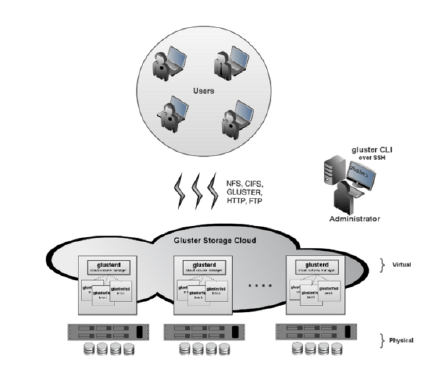
\includegraphics[width=0.7\linewidth]{scheme.png}
	\end{figure}
% GlusterFS is a powerful network/cluster filesystem written in user space which uses FUSE to hook itself with VFS layer.
% GlusterFS takes a layered approach to the file system, where features are added/removed as per the requirement.
% Though GlusterFS is a File System, it uses already tried and tested disk file systems like ext3, ext4, xfs, etc. to store the data.
% It can easily scale up to petabytes of storage which is available to user under a single mount point.
\end{frame}

\begin{frame}{Terms}
	\begin{itemize}
		\item Brick     % The brick is the storage filesystem that has been assigned to a volume.
		\item Subvolume % A brick after being processed by at least one translator.
		\item Volume    % The final share after it passes through all the translators.

		%\item Client
		% The machine which mounts the volume (this may also be a server).
		%\item Server
		% The machine (virtual or bare metal) which hosts the actual filesystem in which data will be stored.

		% \item Translator
		% The brick's first translator (or last, depending on what direction data is flowing) is the storage/posix translator that manages the direct filesystem interface for the rest of the translators.
		% The configuration of translators (since GlusterFS 3.1) is managed through the gluster command line interface (cli), so you don't need to know in what order to graph the translators together.
		% All the translators hooked together to perform a function is called a graph. 		

		\item Trusted storage pool
		% Before you can configure a GlusterFS volume, you must create a trusted storage pool consisting of the
		% storage servers that provides bricks to a volume.
		% A storage pool is a trusted network of storage servers. 
	\end{itemize}
\end{frame}

\begin{frame}{Volume types}
	\begin{itemize}
		\item Distributed
		\item Replicated
		\item Striped
		\vspace{1cm}
		\item Distributed striped
		\item Distributed replicated
		\item Striped replicated
	\end{itemize}
\end{frame}

\begin{frame}{Distributed volumes}
	\begin{figure}[h]
		\centering
		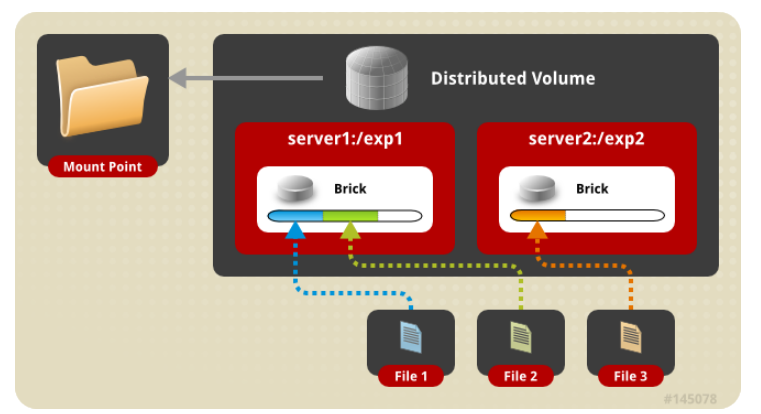
\includegraphics[width=0.8\linewidth]{distributed.png}
	\end{figure}
	% \begin{block}{}
	% 	gluster volume create test-volume server1:/exp1 server2:/exp2
	% \end{block}

	% The server that the files are written to is calculated by hashing the filename.
	% If the filename changes, a pointer file is written to the server that the new hash
	% code would point to, telling the distribute translator which server the file is actually on.
\end{frame}

\begin{frame}{Distributed volumes. Pros and Cons}
	\begin{block}{Advantages}
		\begin{itemize}
			\item More servers - better scaling
			% in terms of random file access. As long as clients aren't all retrieving the same file,
			% their access should be spread pretty evenly across all the servers.
			\item Increasing volume - adding a new server % on-the-fly
		\end{itemize}
	\end{block}
	\begin{block}{Disadvantages}
		\begin{itemize}
			\item Lose of one server - lose access to all its files
			\item File can't be large than subvolume
			\item Filename change -> hashcode not valid -> extra lookup
		\end{itemize}
	\end{block}
\end{frame}

\begin{frame}{Replicated volumes}
	\begin{figure}[h]
		\centering
		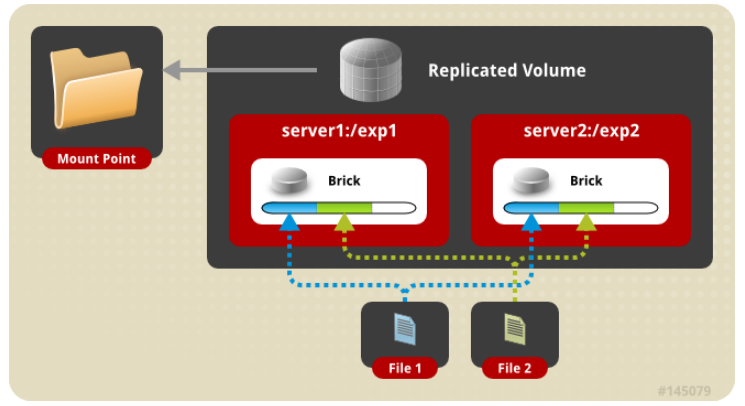
\includegraphics[width=0.8\linewidth]{replicated.png}
	\end{figure}
	% \begin{block}{}
	% 	gluster volume create test-volume replica 2 server1:/exp1 server2:/exp2
	% \end{block}
\end{frame}

\begin{frame}{Striped volumes}
	\begin{figure}[h]
		\centering
		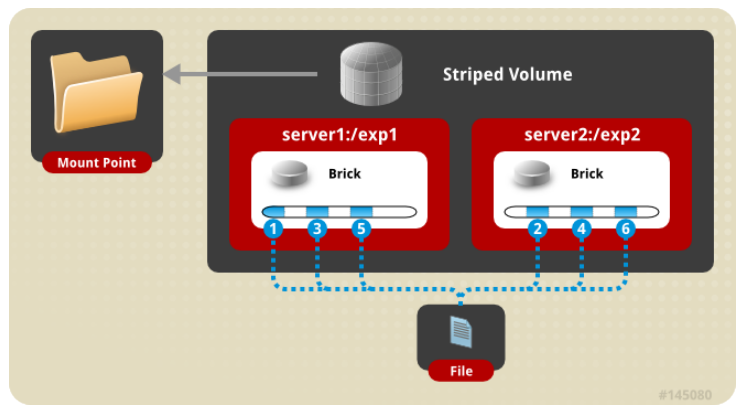
\includegraphics[width=0.8\linewidth]{striped.png}
	\end{figure}
	% \begin{block}{}
	% 	gluster volume create test-volume stripe 2 server1:/exp1 server2:/exp2
	% \end{block}
\end{frame}

\begin{frame}{Setting up (1)}
	\inputminted{bash}{sc1}
	\inputminted{bash}{sc2}
\end{frame}

\begin{frame}{Setting up (2)}
	\inputminted{bash}{sc3}
\end{frame}

\begin{frame}{Performance (1)}
	cat /mnt/Files/example > /dev/null
	700mb
	\begin{block}{NFS}
		0m15.220s

		0m16.139s
		
		0m18.812s
	\end{block}
	\begin{block}{GlusterFS}		
		0m28.101s

		0m20.321s

		0m36.444s
	\end{block}
\end{frame}

\begin{frame}{Performance (2)}
	700 little files, copying
	\begin{block}{NFS}
		0m15.848s

		0m12.792s

		0m13.417s
	\end{block}
	\begin{block}{GlusterFS}
		0m28.318s

		0m27.432s

		0m29.397s
	\end{block}
\end{frame}

\begin{frame}{Performance (3)}
	700 little files, removing
	\begin{block}{NFS}
		0m4.861s

		0m3.618s

		0m4.297s
	\end{block}
	\begin{block}{GlusterFS}
		0m5.050s

		0m7.055s

		0m5.300s
	\end{block}
\end{frame}

\begin{frame}{Links}
	\begin{itemize}
		\item \url{http://www.gluster.org/}
		\item Взрослеем с GlusterFS \url{http://habrahabr.ru/post/140031/}
		\item GlusterFS, опыт новой версии \url{http://habrahabr.ru/post/157029/}
	\end{itemize}
\end{frame}

\end{document}